\ylDisplay{Plaat} % Ülesande nimi
{Tundmatu autor} % Autor
{lahtine} % Voor
{2007} % Aasta
{G 4} % Ülesande nr.
{3} % Raskustase
{
% Teema: Geomeetriline-optika
\ifStatement
Tasaparalleelsel plaadil paksusega $d = \SI{5}{cm}$ on alumine pind hõbetatud. Valguskiir langeb plaadi ülemisele pinnale nurga $\alpha = \SI{30}{\degree}$ all, osaliselt peegeldub sellelt ning osaliselt murdub plaadi sisse. Seejärel peegeldub murdunud kiir plaadi alumiselt pinnalt ning murdub teist korda, väljudes tagasi õhku. Leidke plaadi materjali murdumistegur $n$, kui kaugus esimese peegeldunud ja teise murdunud kiire vahel $l = \SI{2,5}{cm}$.
\fi


\ifHint
Tasub koostada selge joonis ning murdumisnäitaja leidmiseks kasutada täisnurksete kolmnurkade omadusi ja Snelli seadust.
\fi


\ifSolution
Kiirte käik plaadis on näidatud joonisel.

\begin{center}
	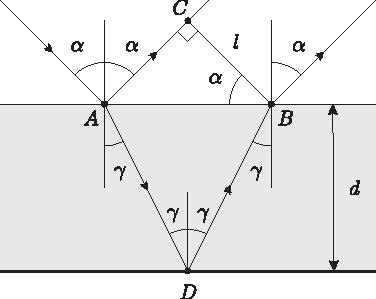
\includegraphics[width=0.7\linewidth]{2007-lahg-04-lah}
\end{center}

Nurk $\angle ABC$ täisnurkses kolmnurgas $ACB$ on $\alpha$, seetõttu $|AB| = l/ \cos \alpha$. Teisest küljest, kolmnurgast $ADB$ on näha, et $|AB| = 2d \tan \gamma$. Nurgad $\alpha$ ja $\gamma$ on seotud omavahel murdumisseadusega:
\[
\frac{\sin\alpha}{\sin\gamma} = n.
\]
Lahendades need võrrandid, saame
\[
n=\frac{\sin\alpha}{\sin\left(\arctan\left(\frac{l}{2d\cos\alpha}\right)\right)} =\sin \alpha \sqrt{1+\left(\frac{2 d \cos \alpha}{l}\right)^{2}} \approx \num{1,8}.
\]
\fi
}